\documentclass[11pt, a4paper]{article}
\usepackage[utf8]{inputenc}
\usepackage{geometry}
\usepackage{graphicx}
\usepackage{float}
\usepackage{amsmath}
\usepackage[dvipsnames]{xcolor}
\geometry{margin=1in}
\setlength{\parindent}{0em}
\setlength{\parskip}{1em}
\title{Computação Gráfica | Trabalho 3}
\author{Professor: Waldemar Celes\\
Aluno: Antenor Barros Leal}
\date{01 de dezembro de 2024}
\begin{document}
\maketitle

\section {Resumo}
Este trabalho tem como objetivo fazer a implementação e teste de técnicas de renderização
em uma cena 3D.

\section {Cena Base}
Para a cena utilizou-se uma versão com leves modificações a partir da tarefa 2.1. 

Para este trabalho o cubo cinza foi retirado para ser substituído por um quad 
que fará papel de uma superfície plana para o refletor e como anteparo para a 
projeção das sombras.

O seguinte grafo de cena foi usado:

\begin{verbatim}
  Node::Make(shader,
      {
          Node::Make(trCube2,{yellow},{cube}),
          Node::Make(trSphere1,{green},{sphere}),
          Node::Make(trSphere2,{red},{sphere}),
          Node::Make(trCube3,{red},{cube}),
      }
  );
\end{verbatim}

\section {Técnicas de Renderização}

Entre as opções, foi escolhida a técnica de reflexão planar e de sombra planar.

\subsection {Técnica: reflexão planar}

Como dito na seção anterior foi usado um quad para "receber" a reflexão que é 
simplesmente a repetição da cena de $y > 0$ em $y < 0$ com a componente y
com sinal trocado. Usando o transformador de escala, conseguimos fazer esta 
inversão vertical:

\begin{verbatim}
trf->Scale(1.0f,-1.0f,1.0f);
\end{verbatim}

Todavia, se apenas isto for feito, a reflexão irá "vazar" para fora da superfície
reflexiva.

\begin{figure}[H]
  \begin{center}
  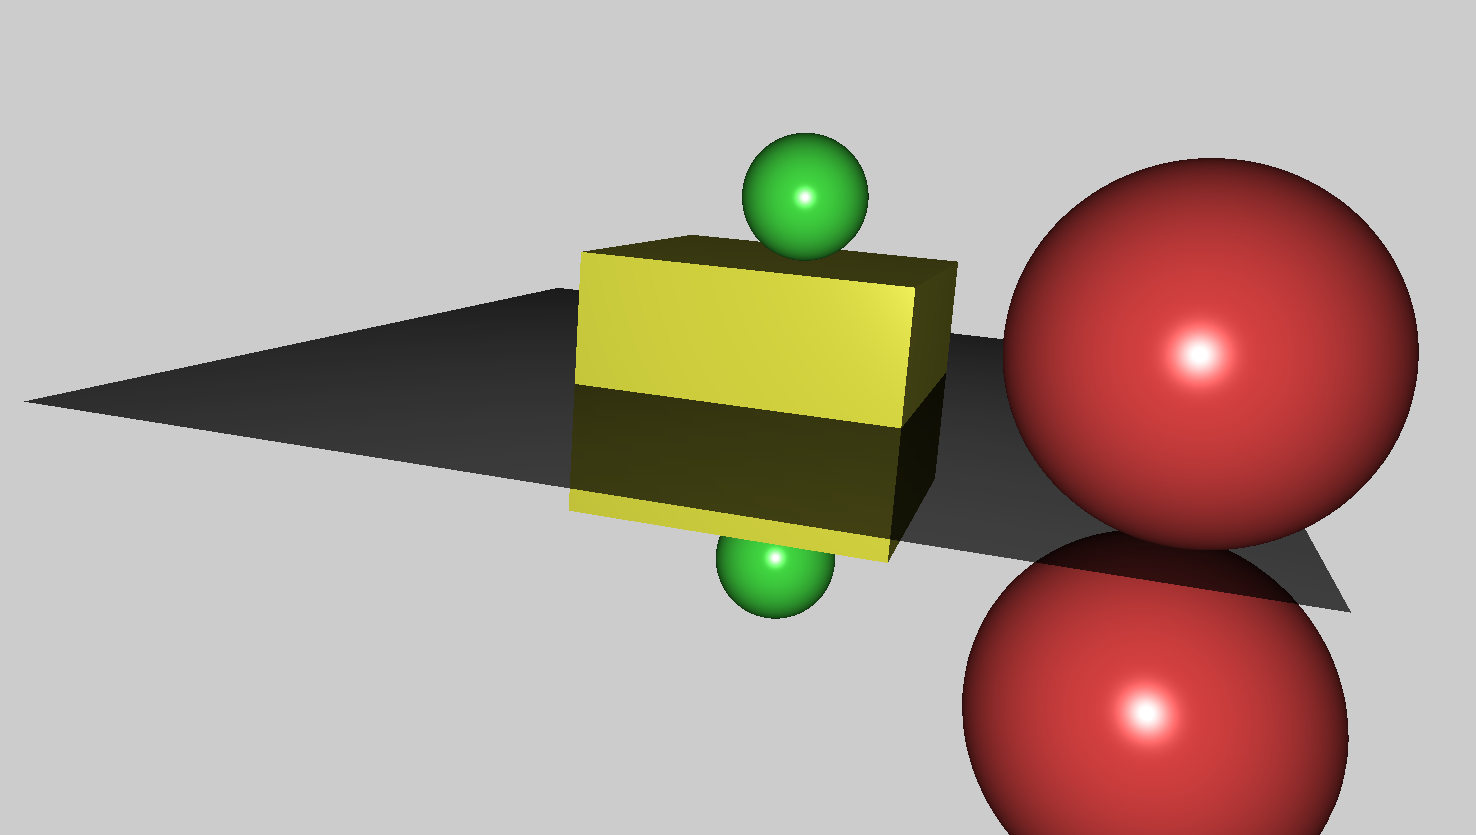
\includegraphics[width=0.8\linewidth]{before-stencil.png}
  \caption{Antes do stencil}
  \label{fig:vaz}
  \end{center}
\end{figure}

Isto é resolvido aplicando um stencil na superficie reflexiva e informando ao 
OpenGL não renderizar a cena que esteja fora desta máscara.

\begin{figure}[H]
  \begin{center}
  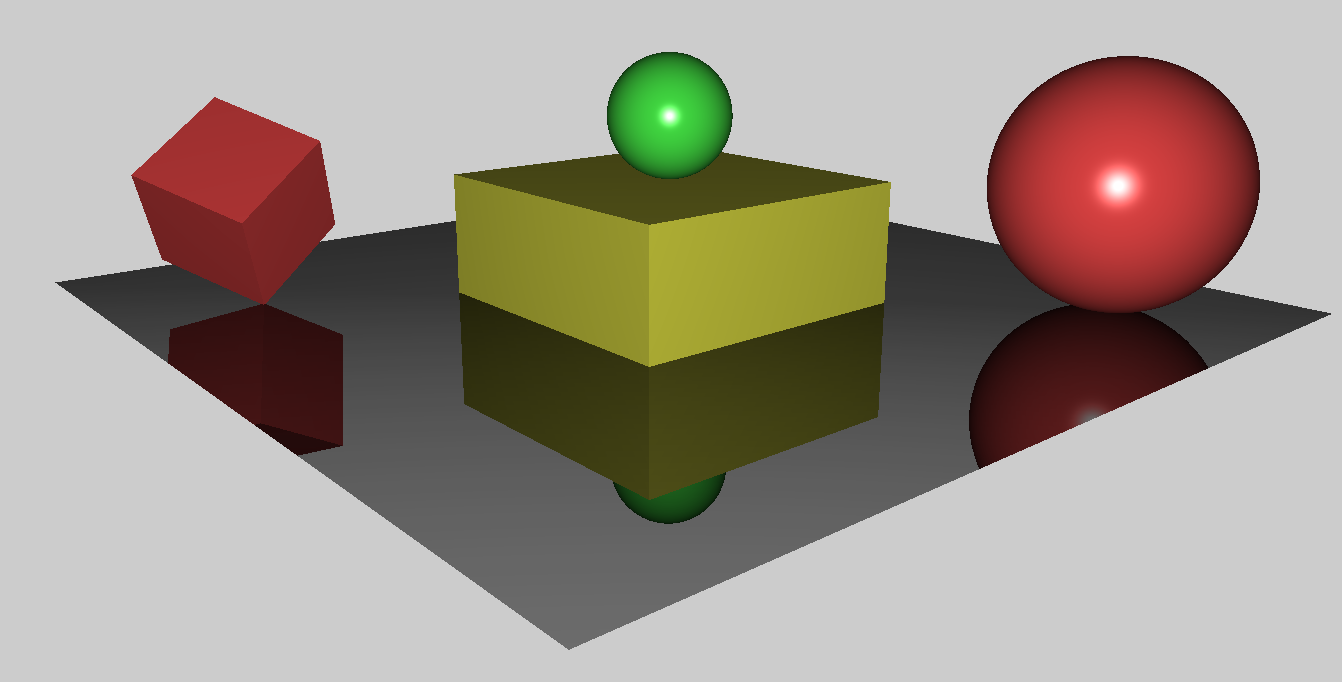
\includegraphics[width=0.8\linewidth]{after-stencil.png}
  \caption{Depois do stencil}
  \label{fig:vaz}
  \end{center}
\end{figure}

Porém se mudarmos o arcball para visualizar a parte de baixo da superficie reflexiva, 
vemos parte do reflexo cortado pelo stencil. O que se é desejado, obviamente, é 
a ausência de qualquer objeto.

\begin{figure}[H]
  \begin{center}
  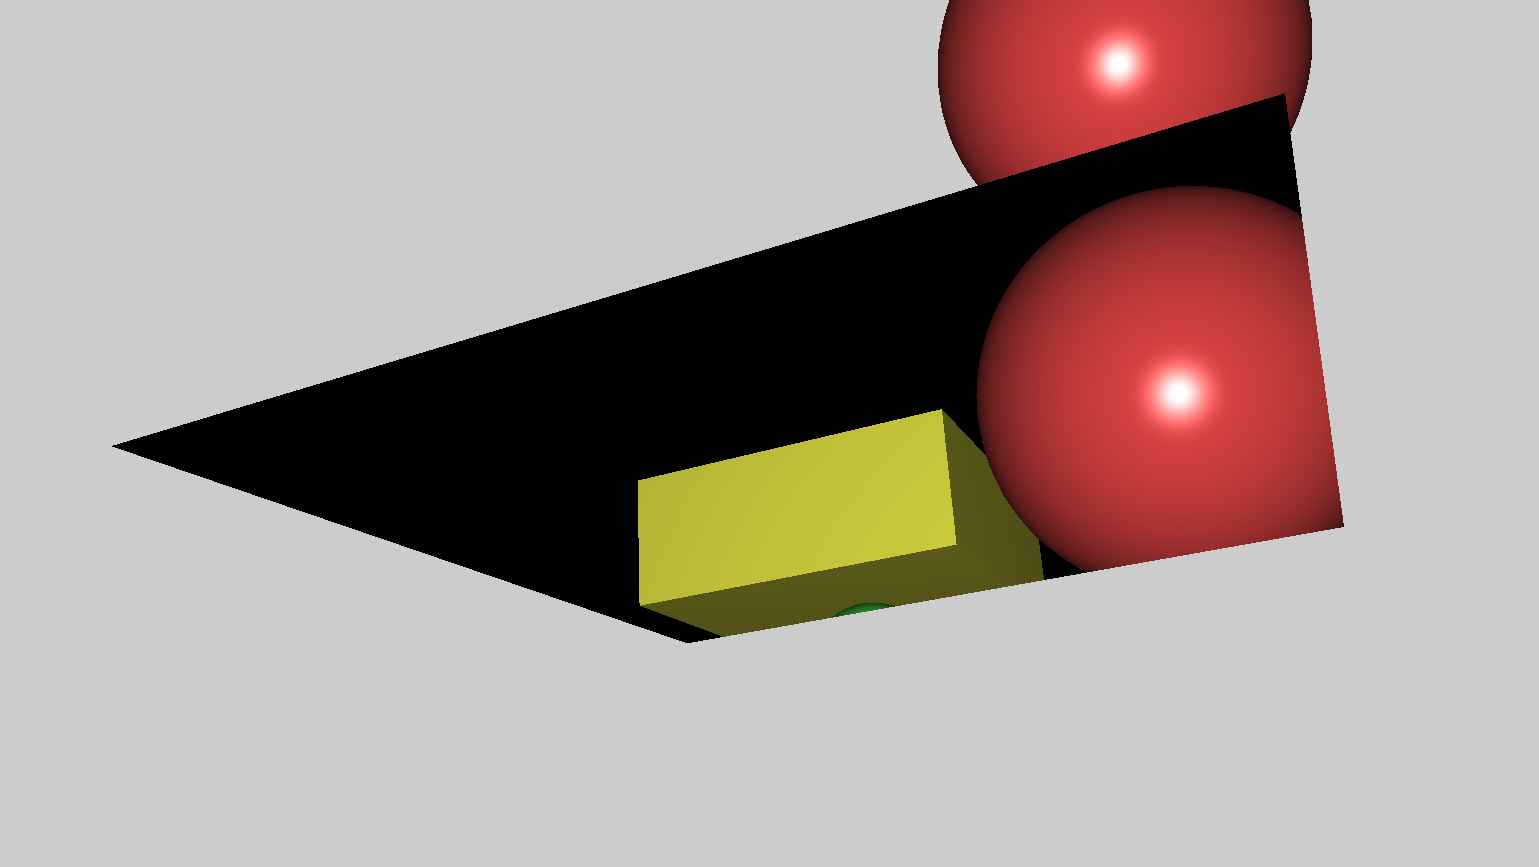
\includegraphics[width=0.8\linewidth]{before-cut-plan.png}
  \caption{Cena refletida aparecendo do outro lado}
  \label{fig:vaz}
  \end{center}
\end{figure}

Para resolver isso, normalmente é usado um plano de corte para mostrar a cena refletida apenas
acima deste plano. Porém não foi conseguido realizar isto. Para contornar, na função
de display é testado se a câmera está no lado de cima do
refletor.
Apenas se este for o caso, a cena refletida aparece.

\begin{verbatim}
if (camera->GetViewMatrix()[1][2] > 0) {
  ...
\end{verbatim}

\begin{figure}[H]
  \begin{center}
  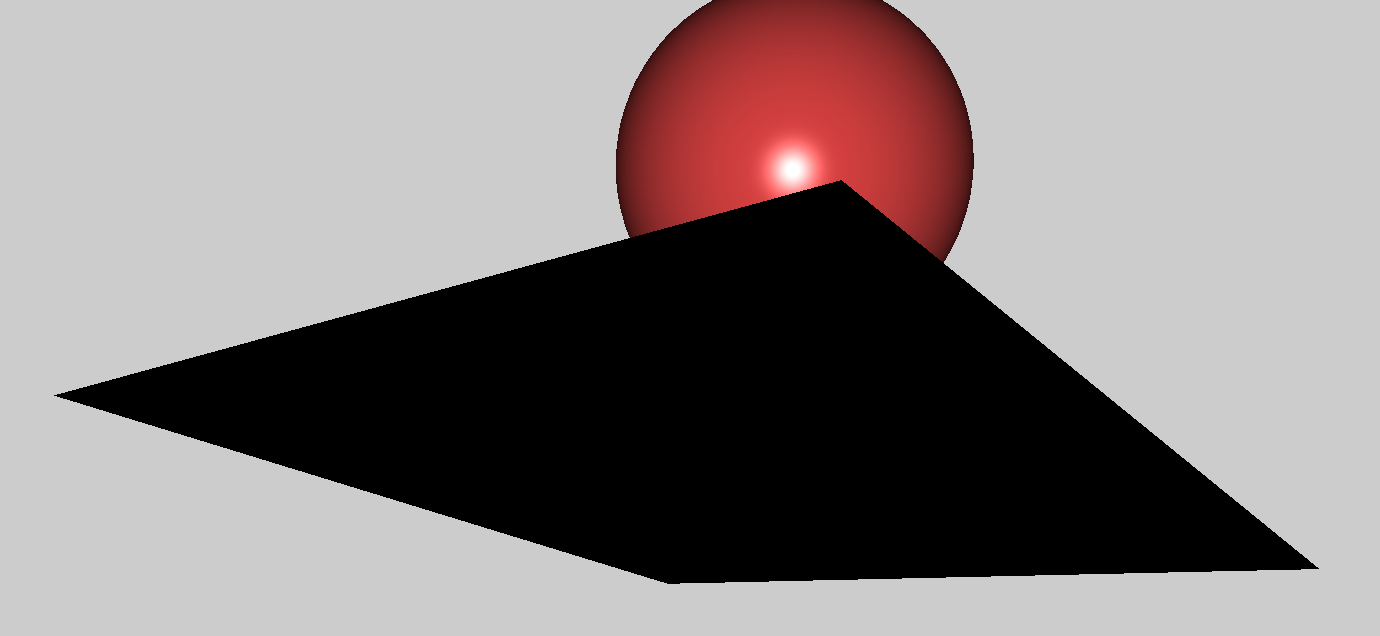
\includegraphics[width=0.8\linewidth]{with-condition.png}
  \caption{Cena corrigida}
  \label{fig:vaz}
  \end{center}
\end{figure}


\subsection {Técnica: sombra planar}

Para a sombra planar, aplicamos a geometria em uma matriz de projeção que "achata"
os objetos de cena em uma superfície 2D. Esta matriz de projeção, por considerar a posição da luz,
consegue simular corretamente como é a sombra projetada por esta luz.

\subsubsection{Matriz de projeção}

\begin{itemize}
\item Seja n o vetor $[n_x n_y n_z]$, representando a normal ao plano onde a sombra deve
ser exibida com os índices iguais às componentes x, y e z.

\item Seja, l o vetor $[l_x l_y l_z ]$ com a posição da fonte de luz.

\item Seja p o vetor $[p_x p_y p_z 1]$ com a posição de um ponto na geometria e
o último índice sempre igual a um.

\end{itemize}

Cada ponto da geometria representado pelo vetor quando for multiplicado pela matriz M.

\[
M = \begin{bmatrix}
  nl + n_{w} - l_{x}n_{x} & -l_{x}n_{y} & -l_{x}n_{z} & -l_{x}n_{w} \\
  -l_{y}n_{x} & nl + n_{w} - l_{y}n_{y} & -l_{y}n_{z} & -l_{y}n_{w} \\
  -l_{z}n_{x} & -l_{z}n_{y} & nl + n_{w} - l_{z}n_{z} & -l_{z}n_{w} \\
  -n_{x} & -n_{y} & -n_{z} & nl
\end{bmatrix}
\]

Será transformado em $p'$, um vetor que representa um ponto no plano da sombra.

$$p' = M p$$

Fazendo esta operação com todos os pontos da geometria, teremos todos os pontos
da sombra.

\subsubsection{Algoritmo}
Para renderizar a cena, faz-se quatro passadas. Inicialmente é limpado o stencil 
porque se não teríamos um efeito de "pintura", já que as marcações do stencil 
iriam se acumular de quadro a quadro.

\begin{verbatim}
glClear(GL_COLOR_BUFFER_BIT | GL_DEPTH_BUFFER_BIT | GL_STENCIL_BUFFER_BIT);
\end{verbatim}

Foi modificado o shader para que fosse possível renderizar a cena apenas com a 
luz ambiente caso uma variável fosse verdadeira.

\begin{verbatim}
if (amb_only) {
  fcolor = ambient;
}
else {
  fcolor = ambient + diffuse + specular;
}
\end{verbatim}

Na primeira passada, é renderizado o chão apenas com a luz ambiente. Isto será
a cor da sombra.

\begin{verbatim}
amb_only->SetValue(true);
sceneGround->Render(camera);
amb_only->SetValue(false);
\end{verbatim}


Na segunda passada, a geometria da cena é multiplicada pela matriz de sombra e o 
stencil é marcado com a resultante. Esta marcação é a sombra.

\begin{verbatim}
glEnable(GL_STENCIL_TEST);
glStencilFunc(GL_NEVER , 1, 0xFFFF);
glStencilOp(GL_REPLACE , GL_REPLACE , GL_REPLACE);
glm::mat4 sm = shadowMatrix(glm::vec4(0.0f,0.0f,1.0f,1.0f),glm::vec4(2.0f, 2.0f, 
10.0f, 1.0f));
TransformPtr tr = Transform::Make();
tr->MultMatrix(sm);
sceneRoot->GetRoot()->SetTransform(tr);
sceneRoot->Render(camera);
sceneRoot->GetRoot()->SetTransform(nullptr);
\end{verbatim}

Na terceira passada, o chão é desenhado normalmente, exceto pelas áreas onde o 
stencil foi marcado. Nestas áreas, apenas a luz ambiente da primeira passada.

\begin{verbatim}
glStencilFunc(GL_EQUAL , 0, 0xFFFF);
glStencilOp(GL_KEEP , GL_KEEP , GL_KEEP);
glBlendFunc(GL_ONE ,GL_ONE);
glEnable(GL_BLEND);
glDepthFunc(GL_EQUAL);
sceneGround->Render(camera);
glDepthFunc(GL_LESS);
glDisable(GL_STENCIL_TEST);
glDisable(GL_BLEND);
\end{verbatim}

Por fim, a cena principal é desenhada normalmente.

\begin{verbatim}
sceneRoot->Render(camera);
\end{verbatim}

\begin{figure}[H]
  \begin{center}
  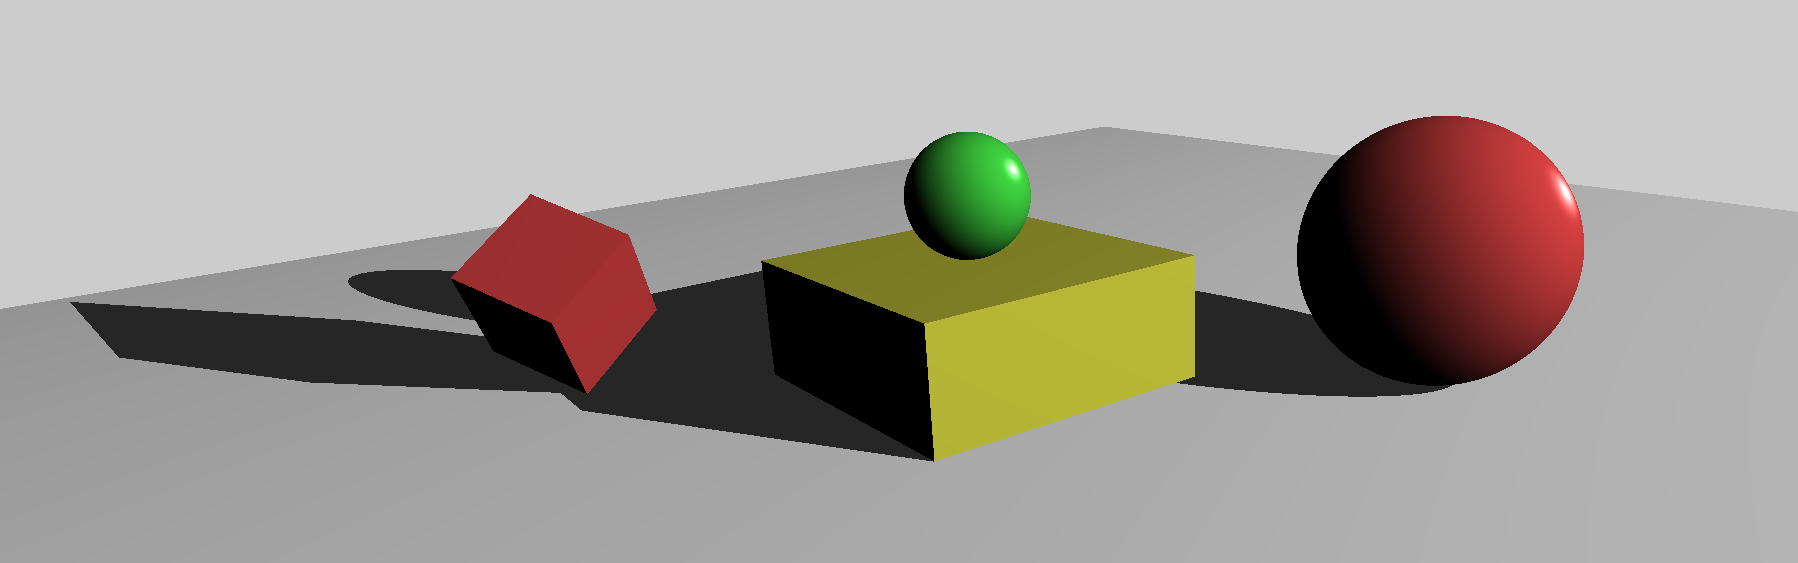
\includegraphics[width=0.8\linewidth]{shadow.png}
  \caption{Cena com sombra}
  \label{fig:vaz}
  \end{center}
\end{figure}

\begin{figure}[H]
  \begin{center}
  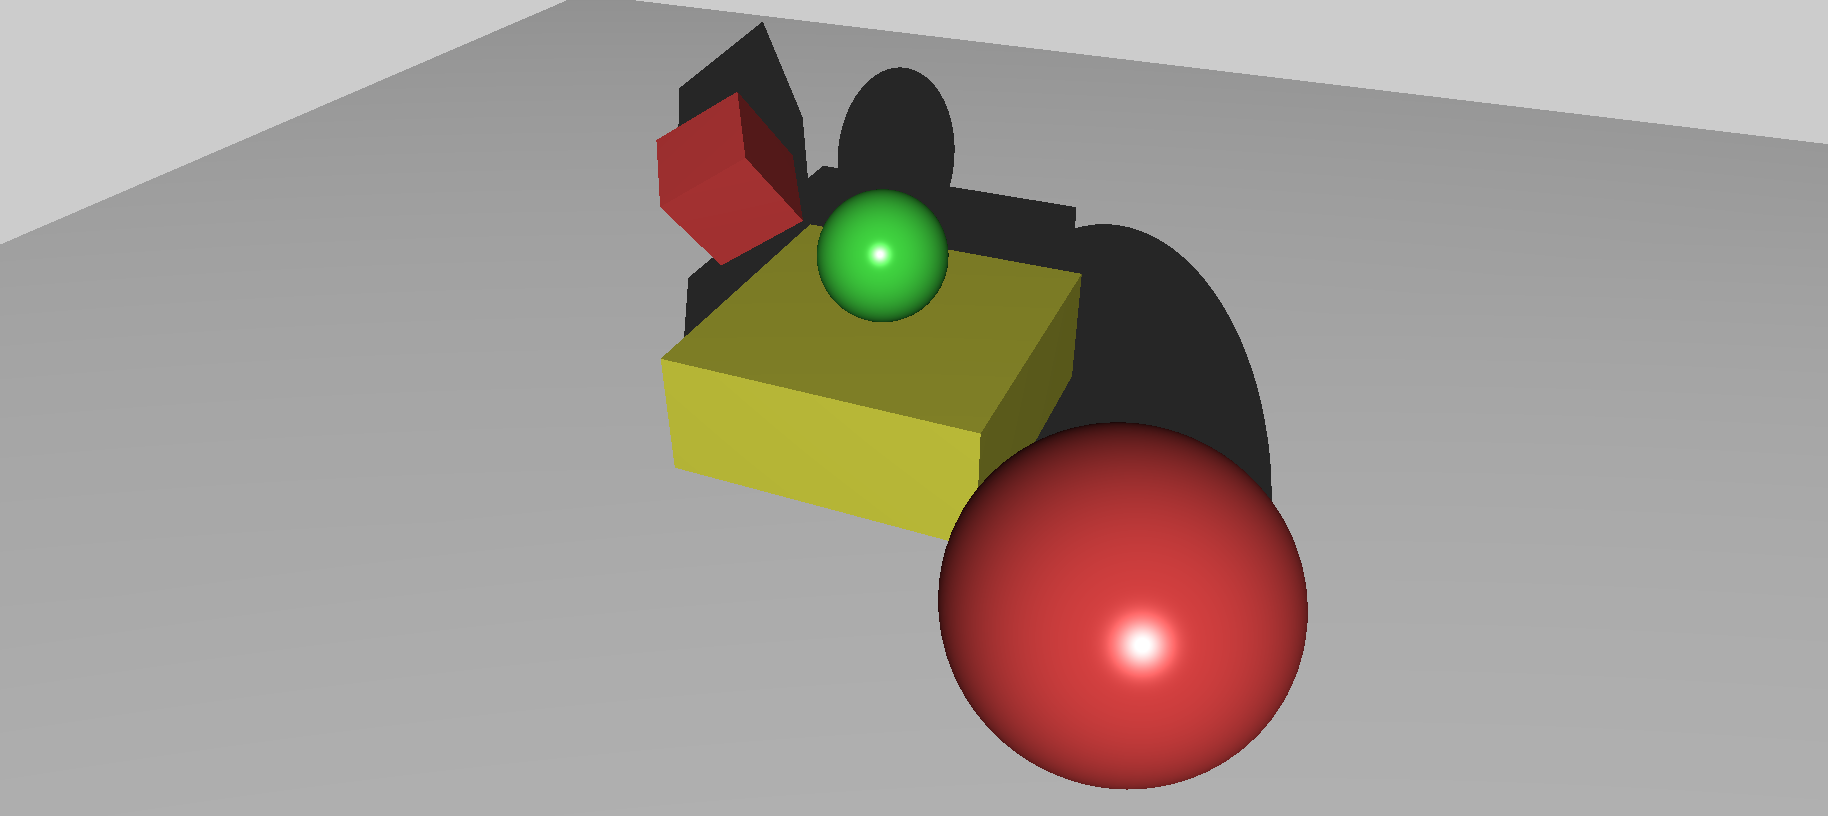
\includegraphics[width=0.8\linewidth]{shadow-2.png}
  \caption{Cena com sombra 2}
  \label{fig:vaz}
  \end{center}
\end{figure}

\section {Resultados}

Além das capturas de tela deste relatório, um vídeo de demostração do funcionamento 
foi incluído no arquivo "demo.mp4".

\end{document}